\section{Videnssamling}
\begin{frame}{Videnssamling}
Vi forsøgte at gøre brug af forskellige teknikker til videnssamling igennem iterationerne:
\begin{itemize}
\item 1 iteration: interview med barer og state of the art
\item 2 iteration: interview med gæster
\item 3 iteration: vertical prototype med fabrikken
\item 4 iteration: usability test på en mobile enhed
\end{itemize}
\end{frame}

\subsection{State Of The Art}
\begin{frame}{State Of The Art}
	Nogle af de koncepter vi fandt fra eksisterende systemer:
	Playlist
	Voting and Requesting
	\begin{itemize}
	\item SecretDJ - Weighted
	\item Mixgar - Limited
	\item Rockbot - Down-voting and indirect requesting
	\end{itemize}

	Gav os en ideer til koncepter der kan bruges bruges denne kontekts.
\end{frame}
\subsection{Interviews og Informanter}
\begin{frame}{Interviews og Informanter}
	Vi gjorde brug af semi-strukturede interviews, for at kunne grave ned i de eksisterende løsningers problemmer, uden at kende systemerne på forhånd.

	Vi valgte at dele interviewsne op i to grupper, der råder over musikken, administratorne, og dem der lytter til musikken i konteksten, gæsterne.

	Derfor tog vi ud på steder, hvor konteksten foregår, altså barer, studiecafeer og lign.

	Dokumentering af interview foregik indskrive hoved emner fra noter og lydoptagelse lavet under interviewsne.

	En bedre forståelse for kontekten og krav til systemet, fra både administratorer og brugerer.
\end{frame}
\subsection{Prototyper}
\begin{frame}{Prototyper}
	\begin{figure}
		\centering
		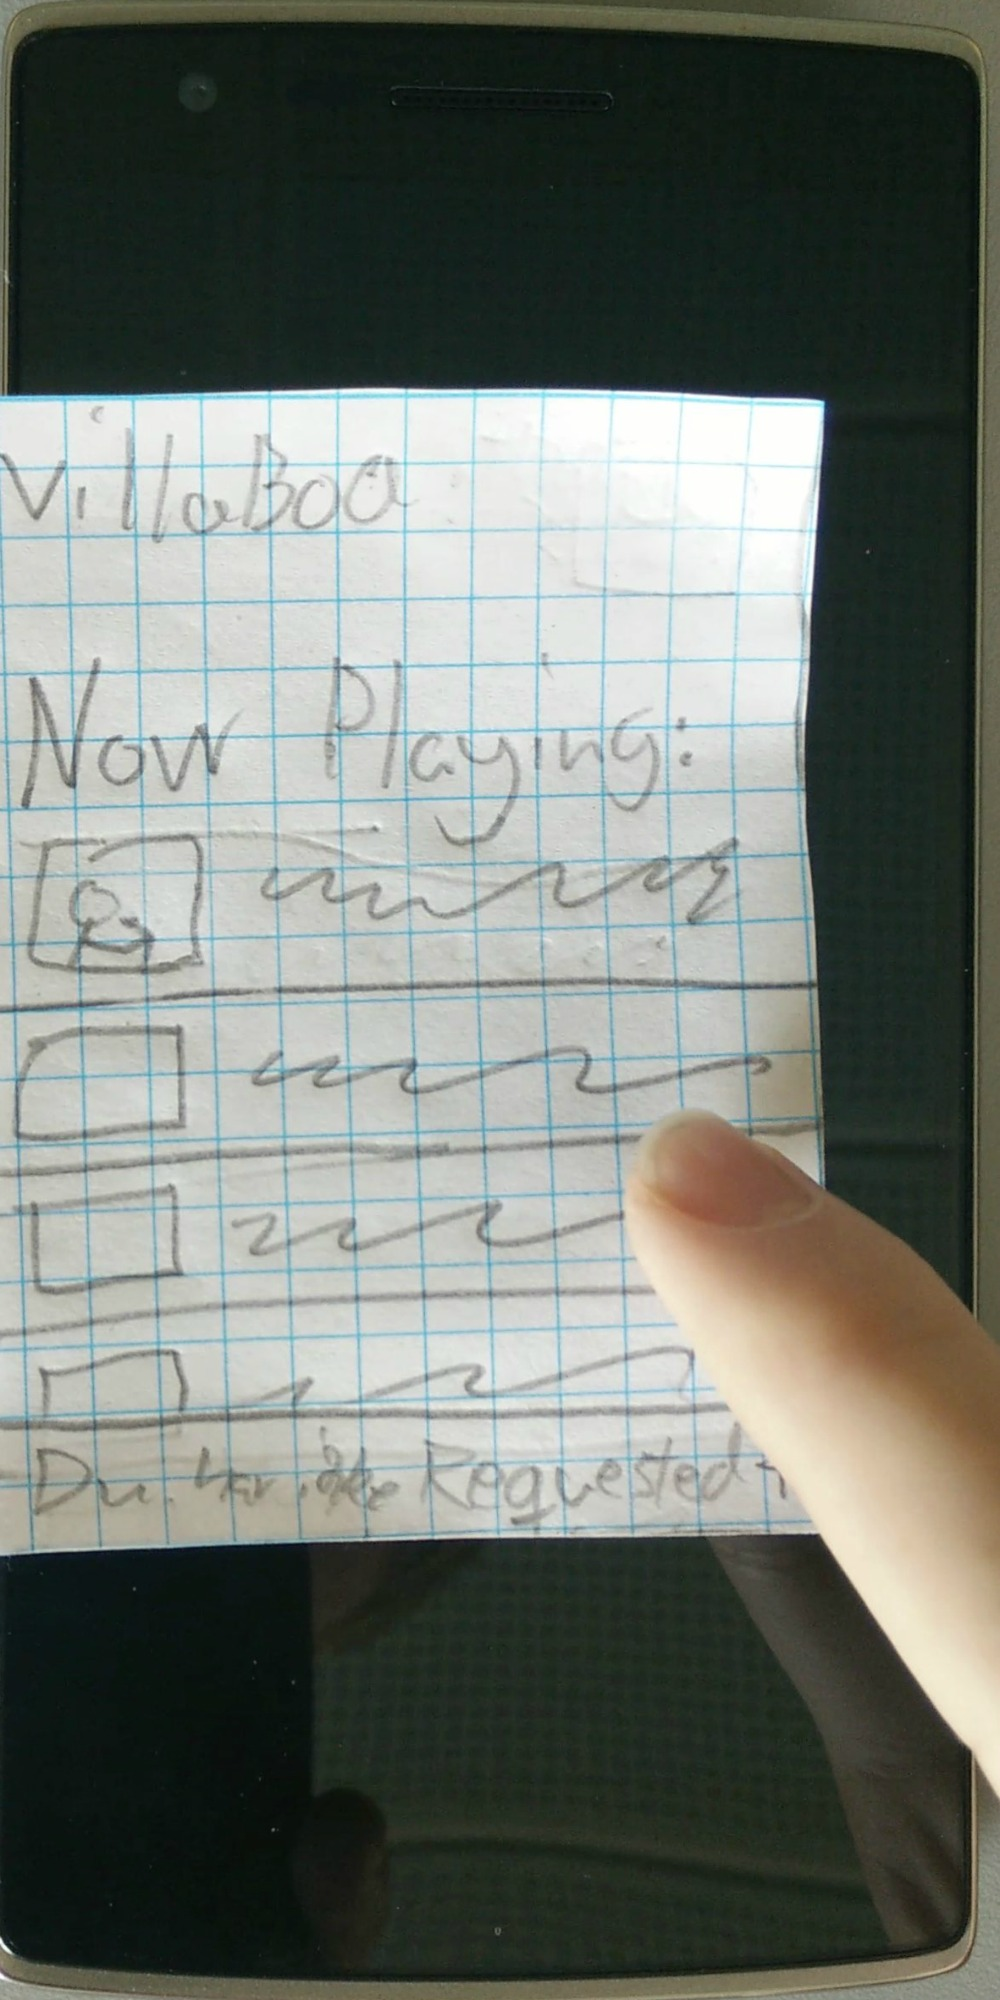
\includegraphics[height=\textwidth/2]{slides/Heider/paperPrototypeVoteInteraction}
		Papirprototype i design phase og i data indsamling en vertical prototype.
	\end{figure}

	Udforskende prototyper til at afprøve nye ideer til design.
	Vertical vurderende prototyper til valg af design og skabelse af nye krav.
\end{frame}
\subsection{Usability test}
\begin{frame}{Usability test}
	\begin{figure}
		\centering
		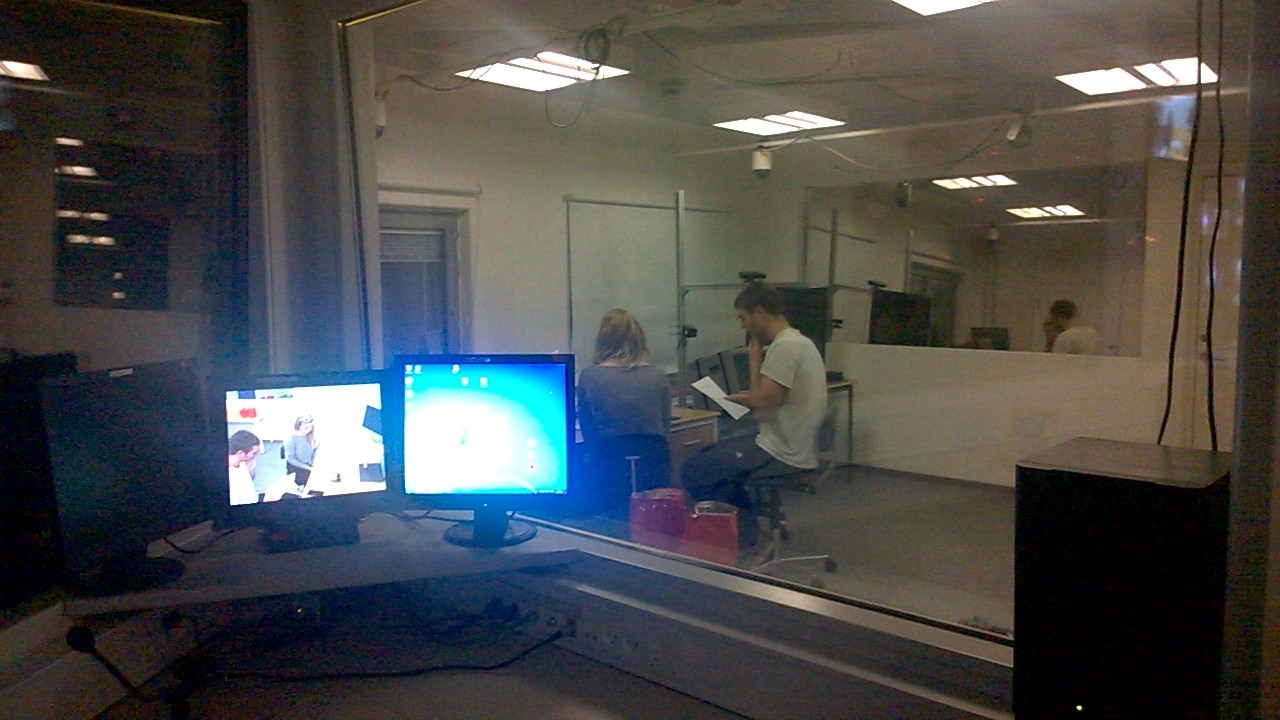
\includegraphics[width=\textwidth/2]{slides/Heider/subjectRoom}
	\end{figure}
	Vi forberedte nogle opgaver som brugerne skulle igennem
	Delte gruppen i nogle roller:
	\begin{itemize}
		\item Datalogger
		\item Leder af testen
		\item Video operatør
		\item Simulator af social interaktion
		\item Underholding og kørsel af test personerne uden for selve testen.
	\end{itemize}
	Til dokumentering brugte vi Instant Data Analysis, da det er hurtigt finde næsten alle problemmerne.

	Gav os indsigt i nogle problemmer med det valgt design og nye krav.
\end{frame}
